\newpage
\section{Experiment}
\subsection{Infrastructure}
\paragraph{}As the experiment's infrastructure, we will describe the frameworks used during the implementation. The framework that has been used to implement the item-based algorithm was Apache Spark. The ALS algorithm was used from the Apache Spark's MLLib library. The framework is common to infrastructure because Apache Spark can orchestrate the work on multiple machines as well as in one. So the framework is as close as we can get to the infrastructure.

\subsubsection{Apache Spark}
\paragraph{}The last decade, analyzing big data is at its peak. Lots of data are produced on daily basis. This means that the need of extracting information from them is raised. 
Lots of frameworks have been used in order to manage and analyze this amount of data. One of the analysis reasons is the need for accurate item recommendations to users. Those items could be movies (e.g. Netflix), music (e.g. Spotify) or products in general(e.g. Amazon). One of the most popular frameworks that could enable this in a distributed way was Apache's Hadoop MapReduce.


\paragraph{}Apache Hadoop has discrete jobs of processing data. The most common jobs are the map and reduce but it has two more jobs, combine and partition. Hadoop has a master node and N worker nodes. The first is responsible to distribute the work, and the second for the work to be done. Each worker usually is called after the job is executing. Hence we have the mapper, the reducer, the partitioner and the combiner. In order to put this to a schema, you can see the figure \ref{hadoopJobsOrder} below.

\begin{figure}[h]
	\centering
	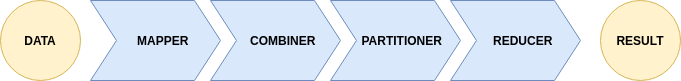
\includegraphics[width=0.5\textwidth]{images/HadoopMapReduceProcesses.png}
	\caption{\bfseries Hadoop Jobs Order}
	\label{hadoopJobsOrder}
\end{figure}

\paragraph{}Hadoop map reduce, is a distributed map-reduce system, 
this means that it has a mechanism to distribute work on nodes and a common interface for handling data. In Hadoop's case, this was able to happen due to Apache Hadoop Yarn and the Hadoop Distributed File System or as commonly used HDFS. When a job was scheduled, data were loaded by the HDFS to a worker, 
then the worker was done, he was putting the result back to the HDFS. 

\paragraph{}As mentioned in \cite{ibmMapReduce:5}, "The term MapReduce actually refers to two separate and distinct tasks that Hadoop programs perform. The first is the map job, which takes a set of data and converts it into another set of data, where individual elements are broken down into tuples (key/value pairs). The reduce job takes the output from a map as input and combines those data tuples into a smaller set of tuples. As the sequence of the name MapReduce implies, the reduce job is always performed after the map job."

\paragraph{}So Hadoop has two basic processes, Map which is responsible for turning the data into key value pairs, and Reduce which takes those pairs and turns them into valuable data.

\paragraph{}If we would like to see where in the DIKW (Data Information Knowledge Wisdom) stack. The Map process would with data and the reduce will end up with information. Of course, this in not always the case, lots of algorithms require lots of cycles in order to complete.
 
\begin{figure}[h]
	\centering
	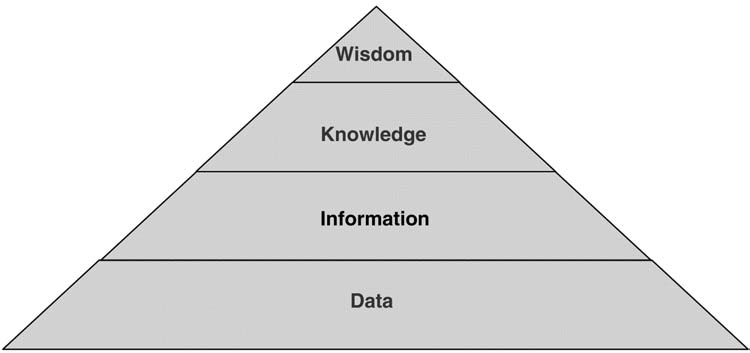
\includegraphics[width=0.5\textwidth]{images/DIKW.png}
	\caption{\bfseries Data Information Knowledge Wisdom Pyramid \cite{TheWisdomHierachy:7}}
	\label{dikw}
\end{figure}
% %note spark version
\paragraph{} But let's make a step back and take a look at Hadoop's architecture. As it is described on its official website \cite{Hadoop:9}, and shown in the figure \ref{hadoopStack} Hadoop uses Hadoop yarn in order to coordinate which process will run on which machine. Also, it uses its file system, the HDFS in order to have a common reference for the files over the network. Last but not least, Hadoop ecosystem is supported by the Hadoop Commons library.

\begin{figure}[h]
	\centering
	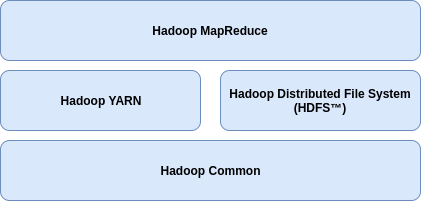
\includegraphics[width=0.5\textwidth]{images/hadoop-stack.png}
	\caption{\bfseries Hadoup Software Stack}
	\label{hadoopStack}
\end{figure}

\paragraph{} In 2009, University of California, Berkley, proposed a new framework for cluster computing in their paper, Spark: Cluster Computing with Working Sets \cite{Zaharia:2010:SCC:1863103.1863113}. They wanted to tackle two major Hadoop issues. 

\paragraph{}The first was the iterative jobs. Each Hadoop job reads from the disk to load data. This means that having iterative jobs, on any given algorithm, you were going to get a large time penalty on reading and of course writing to the disk. 

\paragraph{}The second issue was the interactive analytics. Each Hadoop SQL interface was running as a separate job, and as we mentioned previously we have a big impact on execution time.

\paragraph{}In order to break the acyclic nature of Hadoop, they introduced the Spark's major abstraction, the RDDs. The name RDD stands for Resilient Distributed Datasets. Those datasets are a read-only collection of objects distributed across machines. If a machine fails, the lost part of the RDD can be recalculated. This notion is called lineage.

\paragraph{}Spark is implemented in Scala. Scala is a high-level statically typed programming language. At the time that paper was published, it was believed that Spark was the only system available in a general purpose programming language to make clusters process a large amount of data. As it was mentioned in \cite{Zaharia:2010:SCC:1863103.1863113} "We believe that Spark is the first system to allow an efficient, general purpose programming language to be used interactively to process large datasets on clusters"

\paragraph{}Back to RDDs, an RDD can be created with four different operations as it is described in \cite{Zaharia:2010:SCC:1863103.1863113}. The first operation is loading data from any shared file system. That file system could be HDFS or even an Amazon S3. The second way to create an RDD is by parallelizing any Scala collection. Spark will slice the collection into pieces and distribute it among the nodes. The third way is via transforming an RDD to another one. Because RDDs are immutable, any transformation operation on an RDD, filter, map, flatmap, will generate a new RDD. The last but not least method is by changing an RDDs persistence using save or cache operations.

\paragraph{}Spark also give us the power to do a lot of different distributed operations. Some of them were mentioned before, but we also have operations that would return data to the driver program like collect or reduce. 

\paragraph{}Another important feature of Sparks spine are the shared variables. Spark at its first appearance introduced two of them. The first shared variable is the broadcasted variables. Those variable, RDDs or not, are variables that are commonly used in an algorithm, like a look-up table. By broadcasting a variable, each node gets a copy of the variable in order to access it quickly. The second shared variable that was introduced in that paper was the Accumulators. Those variable live on the spark context, but they can only be increased by any worker and be read from the driver program only. That paper concludes that Spark can outperform Hadoop in some machine learning algorithms and more specific on logistic regression.

\begin{figure}[ht]
  \centering
    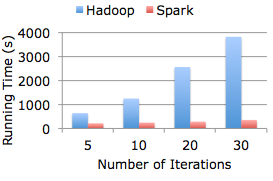
\includegraphics[width=0.5\textwidth]{images/hadoopVsSpark.png}
    \caption{\bfseries Logistic regression, Hadoop vs Spark \cite{HadoopVsSpark}}
   \label{hadoopVsSpark}
\end{figure}

\paragraph{}Coming back to today, Spark's current architecture is depicted below in fig. \ref{apacheSparkStack}. Spark nowadays has an SQL interface in order to search in RDDs with in a query language. Also, Spark support a streaming API to make available real-time analytics. Most of the core machine learning algorithms like ALS, which I used in order to complete this thesis, are the Spark's MLlib component. Finally, the Spark has the component GraphX that is used for handling graphs and graph computation.

\paragraph{}Apache Spark was by design meant to work within Hadoop ecosystem, and most importantly with the HDFS. Apache Spark does not have a file system by itself. You can load data from almost any database, cloud-based or not, even from a local file system. But most will agree that Hadoop and Spark work together just perfect.

\begin{figure}[ht]
  \centering
    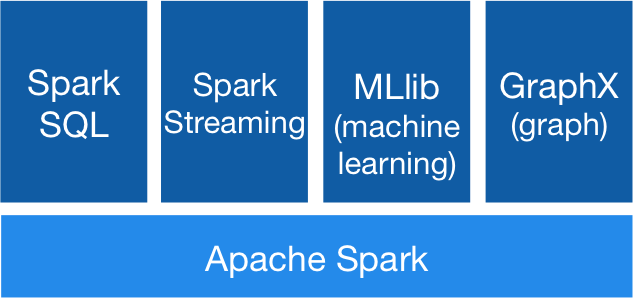
\includegraphics[width=0.5\textwidth]{images/spark-stack.png}
    \caption{\bfseries Apache spark stack \cite{ApacheSpark:1}}
   \label{apacheSparkStack}
\end{figure}

\paragraph{} To conclude, Spark has dominated the big data field the last years, Amazon and other cloud providers give you the option to deploy an Apache Spark cluster on their infrastructure. Also, large companies like Google and Intel are actively contributing to projects like Apache Spark On Kubernetes which can be found at its Github repository \footnote{https://github.com/apache-spark-on-k8s/spark}

\subsection{Dataset}
\paragraph{}Selecting a clear and reliable data set is very important for every experiment in the field. Due to that need several papers, like \cite{levandoski2011recbench}, are using the Movie lens data set. This dataset contains users, movies, and ratings. Each user may rate more than a movie and each movie can be rated by more than one user. The data set split to multiple subsets of 80000 training sets and respective 20000 test set. It also provides scripts that can be used to create more sets.

\paragraph{} In order to better visualize the above dataset, we created an entity relationship(ER) diagram below.
\begin{figure}[ht]
  \centering
    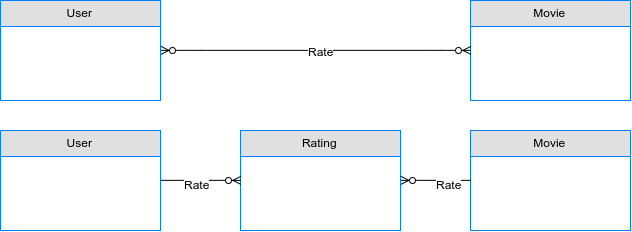
\includegraphics[width=0.5\textwidth]{images/MovieLensDataset.png}
    \caption{\bfseries MovieLens ER diagram \cite{MovieLens:3}}
   \label{movieLensER}
\end{figure}


\subsection{Implementation and assumptions}
\paragraph{}During the implementation, I had to make some assumptions and choices. The first of choices was the framework and the programming language that the implementation would take place. The framework that has been chosen, as you may have already figured out, is apache spark due to its trend and the high scalability it offers. The language of choice was scala, due to its functional nature.
